\documentclass[10pt,a4paper]{article}
\usepackage[utf8]{inputenc}
\usepackage[portuguese]{babel}
\usepackage{amsmath}
\usepackage{amsfonts}
\usepackage{amssymb}
\usepackage{graphicx}
\usepackage{url}
\usepackage{makeidx} 
\usepackage{indentfirst}

\title{\Huge\textbf{Redes Neuronais para Reconhecimento de Linguagem Gestual}\linebreak\linebreak\linebreak
\Large\textbf{Relatório Intercalar}\linebreak\linebreak
\Large{Inteligência Artificial}\linebreak
\Large{3º ano do Mestrado Integrado em Engenharia Informática e Computação} \linebreak \linebreak}
\author{\textbf{Elementos do Grupo:}\\ Diogo Joaquim Pinto – 201108016 - ei11120@fe.up.pt \\ Luís Brochado Pinto dos Reis – 201003074 - ei11009@fe.up.pt \\ Wilson da Silva Oliveira - 201109281 - ei11085@fe.up.pt}
\date{28 de Maio de 2014}

\begin{document}

\begin{figure}
\centering

\includegraphics[width=0.7\linewidth]{./LogoFeup}
\end{figure}

\maketitle

\tableofcontents

\newpage

\section{Objetivo}

Este projeto visa a criação de um programa que seja capaz de aprender e reconhecer a linguagem gestual Australiana  (Auslan), utilizando dados com origem numa camera e num par de luvas com capacidade de efetuar medições de alta precisão, recorrendo às capacidades de aprendizagem não-simbólica das redes neuronais.

\section{Descrição}

\subsection{Dataset}

\subsubsection{Normalização dos dados}

O dataset utilizado para esta aplicação não requeria normalização adicional, uma vez que os dados fornecidos já se encontram normalizados. 

\subsubsection{Parâmetros}

Através da utilização da camera e das luvas de medição foram obtidos onze parâmetros diferentes para cada mão, perfazendo um total de vinte e dois parâmetros que serão processados pela aplicação.

\begin{itemize}
\item Posição X expressa em metros, em relação a uma origem definida ligeiramente abaixo do queixo;
\item Posição Y expressa em metros, em relação a uma origem definida ligeiramente abaixo do queixo;
\item Posição Z expressa em metros, em relação a uma origem definida ligeiramente abaixo do queixo;
\item Rotação no eixo do X, medida num valor entre -0.5 e 0.5, sendo 0 a posição da palma da mão plana horizontalmente. Se o valor for positivo significa que a palma da mão está virada para cima na perspetiva do signatário. Para obter a medida em graus, multiplicar por 180;
\item Rotação no eixo dos Y, medida num valor entre -1.0 e 1.0, sendo 0 a posição da palma para a frente na perspetiva do signatário;
\item Curvatura do dedo polegar medida entre 0 e 1, sendo que 0 significa o dedo esticado e 1 o dedo totalmente dobrado;
\item Curvatura do dedo indicador medida entre 0 e 1, sendo que 0 significa o dedo esticado e 1 o dedo totalmente dobrado;
\item Curvatura do dedo médio medida entre 0 e 1, sendo que 0 significa o dedo esticado e 1 o dedo totalmente dobrado;
\item Curvatura do dedo anelar medida entre 0 e 1, sendo que 0 significa o dedo esticado e 1 o dedo totalmente dobrado;
\item Curvatura do dedo mindinho medida entre 0 e 1, sendo que 0 significa o dedo esticado e 1 o dedo totalmente dobrado.
\end{itemize}
\textbf{É assinalado na fonte da base de dados que as medidas de dobra dos dedos não são totalmente exatas}.

\subsubsection{Processamento do Dataset}

A base de dados contém um total de noventa e cinco palavras com vinte e sete amostras para cada uma totalizando assim dois mil quinhentos e sessenta e cinco amostras.
Cada amostra contém em média sessenta medições únicas (correspondentes aos frames captados pelos dispositivos de medição) dos vinte e dois parâmetros especificados anteriormente.
Dado o elevado número de dados optamos por processar a média destes valores, numa tentativa de reduzir a carga sobre a rede neuronal, mas com o cuidado de garantir valores únicos para cada palavra diferente. Para tentar eliminar os frames menos essenciais para o gesto (que seriam os frames iniciais e finais), optamos por eliminar estes do cálculo da média final.

Para possibilitar o teste da aplicação nos nossos computadores "modestos" utilizamos uma versão reduzida da base de dados com apenas 8 palavras ao invés das 95 disponibilizadas. Não consideramos tal prejudicial visto que isto é uma \textit{proof of concept}

\subsection{Arquitectura da Rede Neuronal}

Existem 3 tipos de de rede neuronal, redes totalmente conectadas, redes de camada única e redes de múltiplas camada.
Optamos pela implementação de \textbf{redes de camada múltipla}, visto que os dados não são linearmente separáveis; e permitiria a implementação de sub-redes, caso o dataset permitisse a associação entre parâmetros, o que levaria a um incremento na eficiência da rede neuronal; e é a qual, dado ser mais comummente utilizada, tem mais heurísticas e recursos desenvolvidos.

As camadas de entrada e de saída possuíam logo à partida valores fixos:
\begin{itemize}
\item a camada de entrada possui 22 nós, um por cada input
\item a camada de saída possui 8 nós (no caso da base de dados reduzida), um por cada palavra
\end{itemize}

Após investigação sobre o tema com especialistas, não foi possível concluir qualquer associação entre os parâmetros relevantes.

Dado isto, foram testadas inúmeras arquiteturas, incluindo redes totalmente conexas com mais e menos nós na camada intermédia, bem como outras topologias: numa delas, como tentativa de agregação de informação, a camada intermédia recebia os dados dos nós da camada de entrada como se segue:
\begin{itemize}
\item posição (x, y, z) das duas mãos
\item dobra dos dedos polegar, indicador e médio da mão esquerda
\item dobra dos dedos polegar, indicador e médio da mão direita
\item dobra dos dedos anelar e mindinho da mão esquerda
\item dobra dos dedos anelar e mindinho da mão direita
\item rotações no espaço da mão esquerda
\item rotações no espaço da mão direita
\item dois nós com todos os parâmetros
\end{itemize}
Após vários testes, acabamos com esta arquitetura como uma das finais: a outra é totalmente conexa e continha uma \textbf{camada intermédia única de 5 nós}.

%TODO : pictures

\subsubsection{Backpropagation}

\begin{figure}[here]
\centering
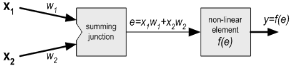
\includegraphics{neuron.png}
\caption{Exemplo de neurónio individual}
\label{Figura 1}
\end{figure}

O algoritmo de backpropagation é um método do tipo feedforward.
Dado isto, inicialmente propaga-se os parâmetros recebidos na camada de entrada pelas ligações. Nas camadas intermédias e na camada de saída, om \textit{impulsos} são somados e em seguida aplica-se uma função de transferência à medida que transmite os dados às camadas seguintes. 

Chegando os \textit{impulsos} à camada de saída, informação é retro-propagada para trás até à camada de entrada: após o cálculo dos erros na camada de saída, os erros são propagados para as camadas intermédias e à medida que o erro vai sendo propagado para trás, o peso das ligações entre camadas é alterado de modo a diminuir o erro. Este passo também é conhecido como "Treino" da rede.

Atualizar o peso das ligações (é equivalente a minimizar o erro) é o modo de se reduzir para zero, ou aproximadamente zero, o erro na camada de saída, tornando a rede neuronal fidedigna.

Este processo é feito através da função de custo quadrático e da sua derivada, sendo que a primeira é a função a minimizar no algoritmo de retropropagação (apresentando \textbf{\textit{x}} exemplos a um rede com \textbf{\textit{y}} saídas).































\subsection{Concepção de uma rede neuronal multi-camada}
\subitem



\subsection{Implementação/aplicação do algoritmo \textit{Back-Propagation}}
\subitem




\subsection{Medição detalhada de resultados nos dados de treino e de teste}
\subitem

Com a arquitetura atual, para 8 palavras a rede demora cerca de 160 iterações pela base de dados para ser propriamente ensinada.

\subsection{Organização do projeto}
\subitem

O trabalho foi dividido em três partes. 
A primeira consiste na criação da rede neuronal e aplicação do algoritmo de retropropagação ("Back-Propagation") e apresentar os resultados bem como as estatísticas.
A segunda parte baseia-se na otimização da primeira parte, de modo a obter respostas mais rapidamente.
A terceira parte trata-se da implementação de funcionalidades adicionais, como por exemplo, uma GUI ou o reconhecimento de gestos através de imagens e/ou vídeo. Esta última parte será posteriormente discutida com os docentes da disciplina.

O grupo está a considerar construir uma rede neuronal modular caso esta se demonstre uma opção útil na otimização do programa. Uma rede neuronal modular atribui determinada tarefa que inicialmente seria desempenhada por um ou vários neurónios, a uma outra "sub" rede neuronal contida na rede principal.
\\ \\

\section{Possíveis Melhorias}
\subsection{Modificação do cálculo do erro}
A inclusão no cálculo do erro de uma iteração de aprendizagem pela rede neuronal da derivada da função sigmóide levaria a uma aprendizagem acelerada nos valores intermédios e lenta perto dos valores limite (0 e 1), sendo que um exemplo já aprendido, no backpropagation não iria alterar em demasia os valores dos pesos, contribuindo para a estabilidade da rede. 

\subsection{Cálculos através da GPU}
Uma hipótese de aumentar a rapidez de treino da base de dados seria implementar a execução dos cálculos através da GPU do computador.

\subsection{Variância como parâmetro}
Uma vez que os dados de input são a média das medições dos parâmetros das amostras, a adição do input das variâncias dos respectivos cálculos poderia ser uma mais valia na distinção entre amostras de movimentos dinâmicos e de estáticos.

\section{Trabalho efetuado}
\subitem

A primeira parte do projeto, enunciada na alínea anterior, já se encontra completa, sendo que o grupo está a iniciar a fase de otimização da rede neuronal, procurando obter um melhor desempenho, e resolver alguns problemas com a mesma.


\section{Resultados esperados e forma de avaliação}
\subitem

À medida que se forem realizando mais testes, o esperado é que o programa a cada chamada necessite de consultar menos pastas da base de dados do que na chamada anterior, pois assim verifica-se que a programa aprendeu o gesto com sucesso e é capaz de o identificar.
Para a utilização da rede neuronal, neste momento é necessário carregar um ficheiro com os valores inseridos manualmente para a rede neuronal poder identifica-lo. Esperamos que até à entrega final nos seja possível implementar uma maneira mais amigável para o utilizador fazer uso desta rede neuronal.

\section{Conclusões}
\subitem

Com este projeto foi possível compreender o conceito de redes neuronais artificiais, bem como as potencialidades da sua utilidade na sociedade. Uma vez que o trabalho ainda não está completo o grupo tem grandes ambições em poder contribuir para a sociedade com este projeto, ajudando a melhorar a perceção de linguagem gestual bem como a identificação de gestos de um modo rápido e eficaz.

\section{Recursos}

O software utilizado foi o IDE IntelliJ IDEA 13.1.1, para programação em Java.


 \begin{thebibliography}{1}

  \bibitem{diapositivos} Eugénio Oliveira {\em Diapositivos de IART: {\url{http://paginas.fe.up.pt/~eol/IA/1314/APONTAMENTOS/7_RN.pdf}}}  2013-2014.
  
  \bibitem{wiki} Wikipedia, Redes Neuronais Modulares {\em\url{http://en.wikipedia.org/wiki/Modular_neural_network}}.

  \bibitem{livroen} Peter Norvig, Stuart Russell {\em Artificial Intelligence A Modern Approach } 2009: Prentice Hall.
  \end{thebibliography}
  \printindex
\end{document}